\chapter{Exodus 36}

\begin{figure}
  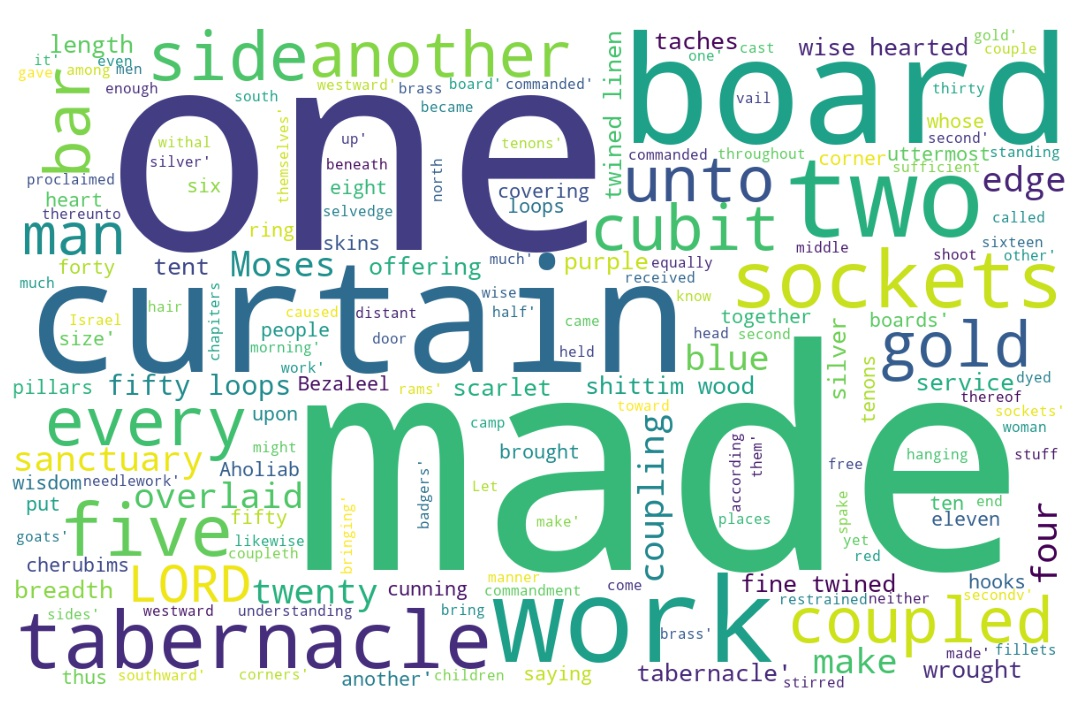
\includegraphics[width=\linewidth]{02OT-Exodus/Exodus36-WordCloud.jpg}
  \caption{Exodus 36 Word Cloud}
  \label{fig:Exodus 36 word Cloud}
\end{figure}

\marginpar{\scriptsize \centering \fcolorbox{bone}{lime}{\textbf{DOING THE WORK}}\\ (Exodus 36:1-38) \begin{compactenum}[I.][8]
    \item An \textbf{Enlightened} Group \index[scripture]{Exodus!Exo 36:01}\index[scripture]{Exodus!Exo 36:02}(Exo 36:1, 2)
    \item \textbf{Envisioned Goal} \index[scripture]{Exodus!Exo 36:02}(Exo 36:2)
    \item \textbf{Excess Giving} \index[scripture]{Exodus!Exo 36:05}(Exo 36:5)
    \item \textbf{Exhibited Grace} \index[scripture]{Exodus!Exo 36:06}(Exo 36:6) 
    \item \textbf{Echoed Guidance} \index[scripture]{Exodus!Exo 36:08-38}(Exo 36:8--38) (repeated for Exodus 26:1--37)
    \item \textbf{Employed Gold} \index[scripture]{Exodus!Exo 36:34}\index[scripture]{Exodus!Exo 36:36}(Exo 36:34, 36)
\end{compactenum}}










\footnote{\textcolor[cmyk]{0.99998,1,0,0}{\hyperlink{TOC}{Return to end of Table of Contents.}}}\footnote{\href{https://audiobible.com/bible/exodus_36.html}{\textcolor[cmyk]{0.99998,1,0,0}{Exodus 36 Audio}}}\textcolor[cmyk]{0.99998,1,0,0}{Then wrought Bezaleel and Aholiab, and every wise hearted man, in whom \fcolorbox{bone}{lime}{the LORD put wisdom and understanding} to know how to work all manner of work for the service of the sanctuary, according to all that the LORD had commanded.}
[2] \textcolor[cmyk]{0.99998,1,0,0}{And Moses called Bezaleel and Aholiab, and every wise hearted man, in whose heart the LORD \fcolorbox{bone}{lime}{had put wisdom}, \emph{even} every one whose heart \fcolorbox{bone}{lime}{stirred} him up to come unto the work to do it:}
[3] \textcolor[cmyk]{0.99998,1,0,0}{And they received of Moses all the offering, which the children of Israel had brought for the work of the service of the sanctuary, to make it \emph{withal}. And they brought yet unto him free offerings every morning.}
[4] \textcolor[cmyk]{0.99998,1,0,0}{And all the wise men, that wrought all the work of the sanctuary, came every man from his work which they made;}\\
\\
\P \textcolor[cmyk]{0.99998,1,0,0}{And they spake unto Moses, saying, The people bring much \fcolorbox{bone}{lime}{more than} \fcolorbox{bone}{lime}{enough} for the service of the work, which the LORD commanded to make.}
[6] \textcolor[cmyk]{0.99998,1,0,0}{And Moses gave commandment, and they caused it to be proclaimed throughout the camp, saying, Let neither man nor woman make any more work for the offering of the sanctuary. So the people were \fcolorbox{bone}{lime}{restrained} from bringing.}
[7] \textcolor[cmyk]{0.99998,1,0,0}{For the stuff they had was sufficient for all the work to make it, and too much.}\\
\\
\P \textcolor[cmyk]{0.99998,1,0,0}{And every wise hearted man among them that wrought the work of the \fcolorbox{bone}{bone}{tabernacle} made ten curtains \emph{of} fine twined linen, and blue, and purple, and scarlet: \emph{with} cherubims of cunning work made he them.}
[9] \textcolor[cmyk]{0.99998,1,0,0}{The length of one curtain \emph{was} twenty and eight cubits, and the breadth of one curtain four cubits: the curtains \emph{were} all of one size.}
[10] \textcolor[cmyk]{0.99998,1,0,0}{And he coupled the five curtains one unto another: and \emph{the} \emph{other} five curtains he coupled one unto another.}
[11] \textcolor[cmyk]{0.99998,1,0,0}{\fcolorbox{bone}{bone}{And he made} loops of blue on the edge of one curtain from the selvedge in the coupling: likewise he made in the uttermost side of \emph{another} curtain, in the coupling of the second.}
[12] \textcolor[cmyk]{0.99998,1,0,0}{Fifty loops made he in one curtain, and fifty loops made he in the edge of the curtain which \emph{was} in the coupling of the second: the loops held one \emph{curtain} to another.}
[13] \textcolor[cmyk]{0.99998,1,0,0}{\fcolorbox{bone}{bone}{And he made} fifty taches of gold, and coupled the curtains one unto another with the taches: so it became one \fcolorbox{bone}{bone}{tabernacle}.}\\
\\
\P \textcolor[cmyk]{0.99998,1,0,0}{\fcolorbox{bone}{bone}{And he made} curtains \emph{of} goats' \emph{hair} for the tent over the \fcolorbox{bone}{bone}{tabernacle}: eleven curtains he made them.}
[15] \textcolor[cmyk]{0.99998,1,0,0}{The length of one curtain \emph{was} thirty cubits, and four cubits \emph{was} the breadth of one curtain: the eleven curtains \emph{were} of one size.}
[16] \textcolor[cmyk]{0.99998,1,0,0}{And he coupled five curtains by themselves, and six curtains by themselves.}
[17] \textcolor[cmyk]{0.99998,1,0,0}{\fcolorbox{bone}{bone}{And he made} fifty loops upon the uttermost edge of the curtain in the coupling, and fifty loops made he upon the edge of the curtain which coupleth the second.}
[18] \textcolor[cmyk]{0.99998,1,0,0}{\fcolorbox{bone}{bone}{And he made} fifty taches \emph{of} brass to couple the tent together, that it might be one.}
[19] \textcolor[cmyk]{0.99998,1,0,0}{\fcolorbox{bone}{bone}{And he made} a covering for the tent \emph{of} rams' skins dyed red, and a covering \emph{of} badgers' skins above \emph{that}.}\\
\\
\P \textcolor[cmyk]{0.99998,1,0,0}{\fcolorbox{bone}{bone}{And he made} boards for the \fcolorbox{bone}{bone}{tabernacle} \emph{of} shittim wood, standing up.}
[21] \textcolor[cmyk]{0.99998,1,0,0}{The length of a board \emph{was} ten cubits, and the breadth of a board one cubit and a half.}
[22] \textcolor[cmyk]{0.99998,1,0,0}{One board had two tenons, equally distant one from another: thus did he make for all the boards of the \fcolorbox{bone}{bone}{tabernacle}.}
[23] \textcolor[cmyk]{0.99998,1,0,0}{\fcolorbox{bone}{bone}{And he made} boards for the \fcolorbox{bone}{bone}{tabernacle}; twenty boards for the south side southward:}
[24] \textcolor[cmyk]{0.99998,1,0,0}{And forty sockets of silver he made under the twenty boards; two sockets under one board for his two tenons, and two sockets under another board for his two tenons.}
[25] \textcolor[cmyk]{0.99998,1,0,0}{And for the other side of the \fcolorbox{bone}{bone}{tabernacle}, \emph{which} \emph{is} toward the north corner, he made twenty boards,}
[26] \textcolor[cmyk]{0.99998,1,0,0}{And their forty sockets of silver; two sockets under one board, and two sockets under another board.}
[27] \textcolor[cmyk]{0.99998,1,0,0}{And for the sides of the \fcolorbox{bone}{bone}{tabernacle} westward he made six boards.}
[28] \textcolor[cmyk]{0.99998,1,0,0}{And two boards made he for the corners of the \fcolorbox{bone}{bone}{tabernacle} in the two sides.}
[29] \textcolor[cmyk]{0.99998,1,0,0}{And they were coupled beneath, and coupled together at the head thereof, to one ring: thus he did to both of them in both the corners.}
[30] \textcolor[cmyk]{0.99998,1,0,0}{And there were eight boards; and their sockets \emph{were} sixteen sockets of silver, under every board two sockets.}\\
\\
\P \textcolor[cmyk]{0.99998,1,0,0}{\fcolorbox{bone}{bone}{And he made} bars of shittim wood; five for the boards of the one side of the \fcolorbox{bone}{bone}{tabernacle},}
[32] \textcolor[cmyk]{0.99998,1,0,0}{And five bars for the boards of the other side of the \fcolorbox{bone}{bone}{tabernacle}, and five bars for the boards of the \fcolorbox{bone}{bone}{tabernacle} for the sides westward.}
[33] \textcolor[cmyk]{0.99998,1,0,0}{\fcolorbox{bone}{bone}{And he made} the middle bar to shoot through the boards from the one end to the other.}
[34] \textcolor[cmyk]{0.99998,1,0,0}{And he overlaid the boards with \fcolorbox{bone}{lime}{gold}, and made their rings \emph{of} gold \emph{to} \emph{be} places for the bars, and overlaid the bars with \fcolorbox{bone}{lime}{gold}.}\\
\\
\P \textcolor[cmyk]{0.99998,1,0,0}{\fcolorbox{bone}{bone}{And he made} a vail \emph{of} blue, and purple, and scarlet, and fine twined linen: \emph{with} cherubims made he it of cunning work.}
[36] \textcolor[cmyk]{0.99998,1,0,0}{\fcolorbox{bone}{bone}{And he made} thereunto four pillars \emph{of} shittim \emph{wood}, and overlaid them with gold: their hooks \emph{were} \emph{of} \fcolorbox{bone}{lime}{gold}; and he cast for them four sockets of silver.}\\
\\
\P \textcolor[cmyk]{0.99998,1,0,0}{\fcolorbox{bone}{bone}{And he made} an hanging for the \fcolorbox{bone}{bone}{tabernacle} door \emph{of} blue, and purple, and scarlet, and fine twined linen, of needlework;}
[38] \textcolor[cmyk]{0.99998,1,0,0}{And the five pillars of it with their hooks: and he overlaid their chapiters and their fillets with gold: but their five sockets \emph{were} \emph{of} brass.}